% !TEX encoding = cp1250
\chapter{Projekt}



\section{Sprawdzenie poprawno�ci punktu pracy}

Implementacja zadania znajduje si� w pliku \texttt{zad1\_2.m}.

Punkt pracy r�wny jest $U_{pp} = 0$, $Y_{pp} = 0$, co zosta�o przedstawione na wykresach \ref{zad1_u} i \ref{zad1_y}.

\begin{figure}[H]
	\centering
	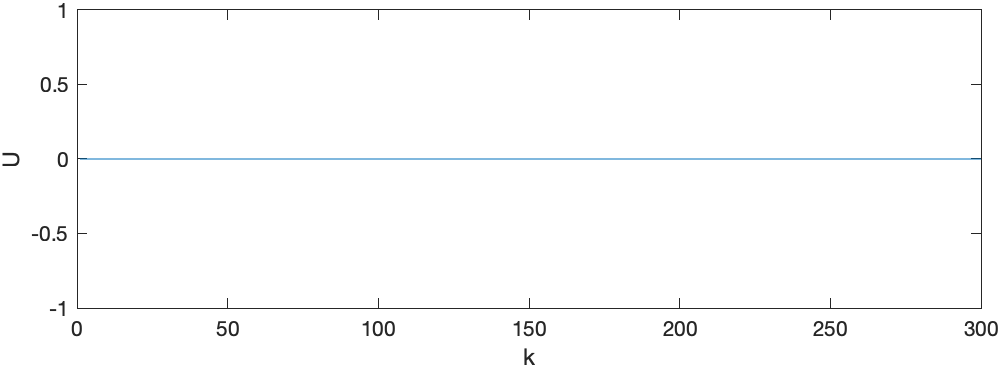
\includegraphics[scale=0.75]{png/projekt/zad1_u.png}
	\caption{Wej�cie uk�adu w punkcie pracy}
	\label{zad1_u}
\end{figure}

\begin{figure}[H]
	\centering
	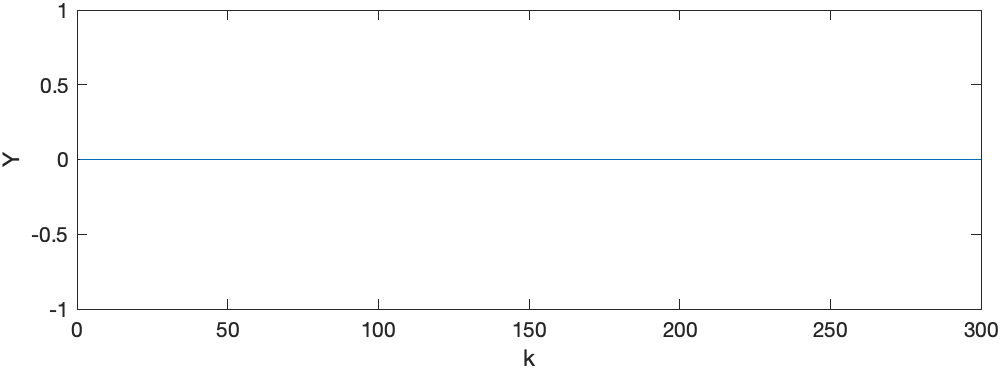
\includegraphics[scale=0.75]{png/projekt/zad1_y.png}
	\caption{Wyj�cie uk�adu w punkcie pracy}
	\label{zad1_y}
\end{figure}

 
\section{Wyznaczenie odpowiedzi skokowych procesu}

Uk�ad zosta� pobudzony sygna�ami o warto�ciach $ U = [-0,8; -0,3; 0,2; 0,6; 1,0]$.

Otrzymane zosta�y w ten spos�b odpowiedzi skokowe:

\begin{figure}[H]
	\centering
	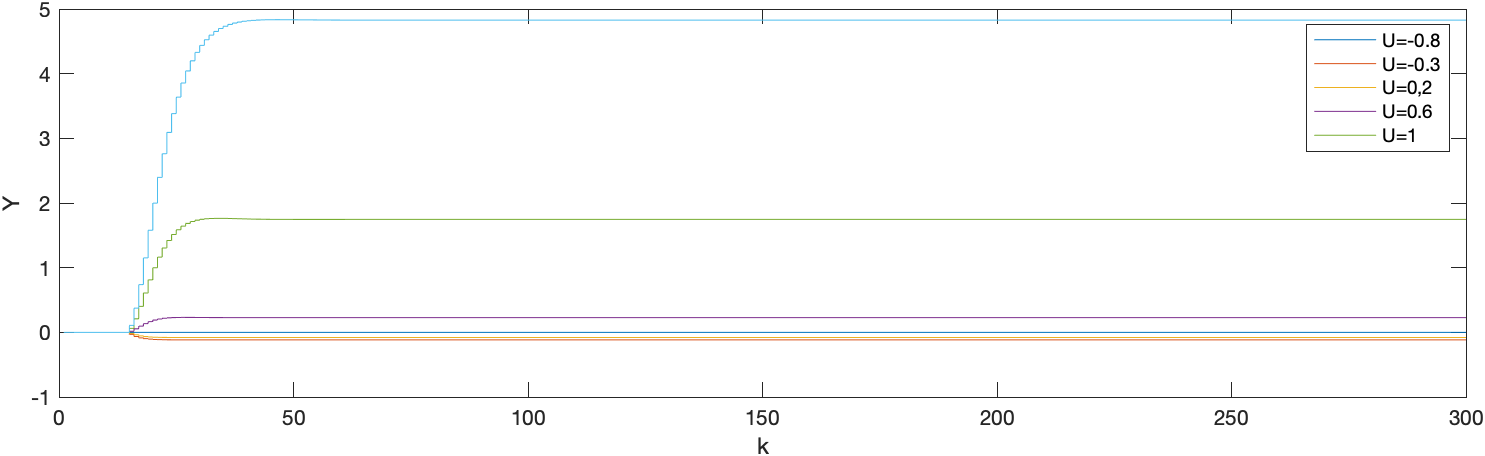
\includegraphics[scale=0.6]{png/projekt/zad2_1.png}
	\caption{Otrzymane odpowiedzi skokowe}
	\label{zad2_1}
\end{figure}

Na wykresie  \ref{zad2_2}  widoczna jest charakterystyka statyczna obiektu.

\begin{figure}[H]
	\centering
	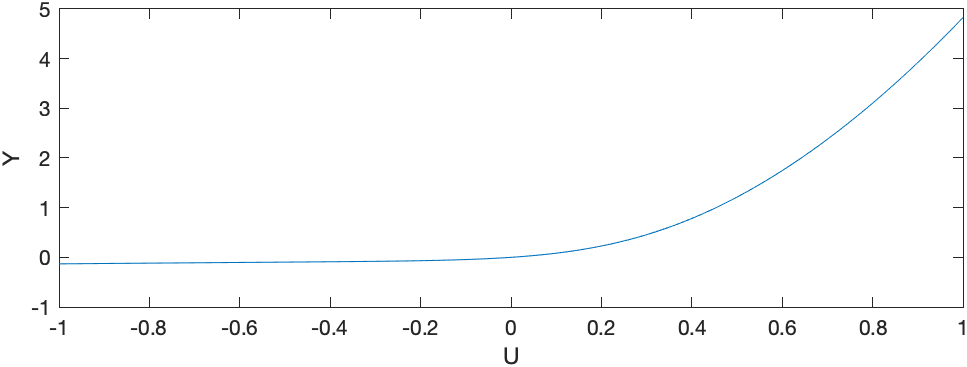
\includegraphics[scale=0.75]{png/projekt/zad2_2.png}
	\caption{Charakterystyka statyczna}
	\label{zad2_2}
\end{figure}

W�a�ciwo�ci dynamiczne oraz statyczne nie s� liniowe. Do charakterystyki statycznej nie mo�e zosta� dopasowana prosta.

\section{Algorytmy PID i DMC}

Obiekt zosta� poddany regulacji za pomoc� algorytm�w PID i DMC z Projektu 2.

TODO opis PID, DMC

\begin{figure}[H]
	\centering
	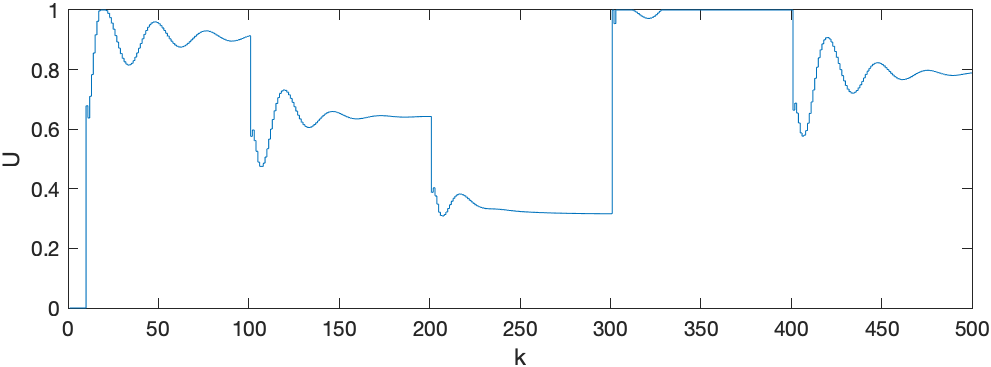
\includegraphics[scale=0.75]{png/projekt/zad3_pid_u.png}
	\caption{Wej�cie uk�adu - algorytm PID}
	\label{zad3_pid_u}
\end{figure}

\begin{figure}[H]
	\centering
	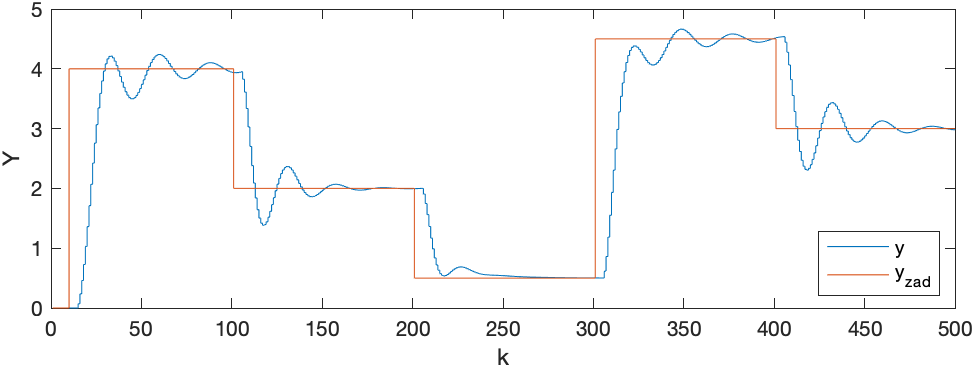
\includegraphics[scale=0.75]{png/projekt/zad3_pid_y.png}
	\caption{Wyj�cie uk�adu - algorytm PID}
	\label{zad3_pid_y}
\end{figure}

\begin{figure}[H]
	\centering
	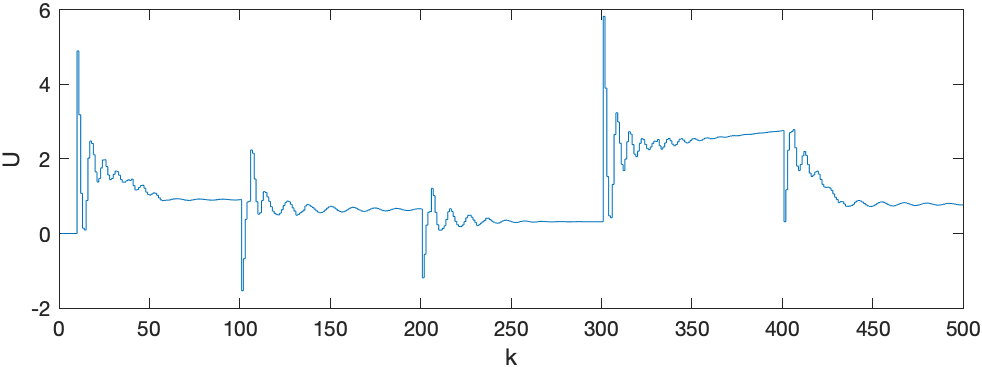
\includegraphics[scale=0.75]{png/projekt/zad3_dmc_u.png}
	\caption{Wej�cie uk�adu - algorytm PID}
	\label{zad3_dmc_u}
\end{figure}

\begin{figure}[H]
	\centering
	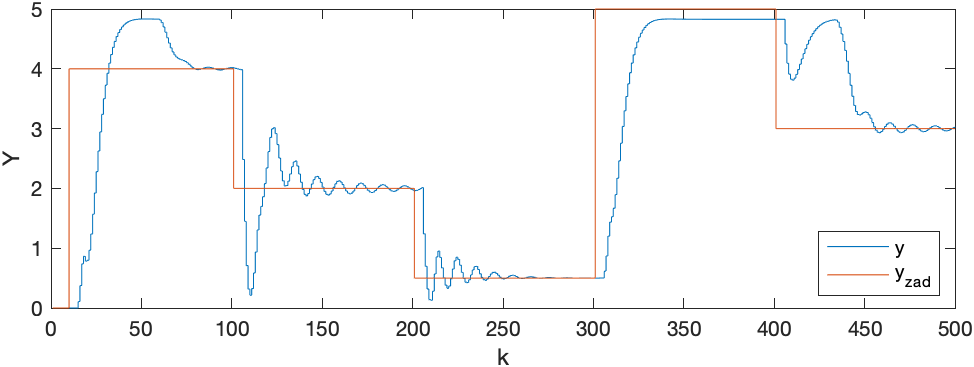
\includegraphics[scale=0.75]{png/projekt/zad3_dmc_y.png}
	\caption{Wyj�cie uk�adu - algorytm PID}
	\label{zad3_dmc_y}
\end{figure}



\section{Rozmyty algorytm PID}

\section{Rozmyty algorytm DMC}

